\input{sep3-annotated-ott}
\input{sep3-unannotated-ott}

\renewcommand{\Sepdrulename}[1]{\scriptsize \textsc{#1}}
\renewcommand{\SepUdrulename}[1]{\scriptsize \textsc{#1}}
% See the seppp.tex file for reminders of the motivation of the
% design.

The previous chapter introduced the freedom of speech
dependently-typed functional programming language. This language
contains two fragments, the logical fragment and the programmatic
fragment.  However, these fragments are judgmentally kept separate.
That is, the syntax was the same for both fragments, even more so, the
syntax for programs and types are collapsed into a single syntactic
category.  This particular design is very appealing because it has an
elegant definition, but this elegance comes at a cost.  The type
system suffers from many value restrictions, and as we have said
above, this makes programming very hard.

Consider a design where instead of a judgmental separation of the two
fragments -- logical and programmatic -- we insist on a syntactic one.
This means that the logical and programmatic fragments have completely
distinct languages for types and programs -- but their semantics are
not -- and then the two fragments are related using freedom of
speech\index{Freedom of Speech} by typing rules.  So we go from a
picture that looks like this:
\begin{center}
  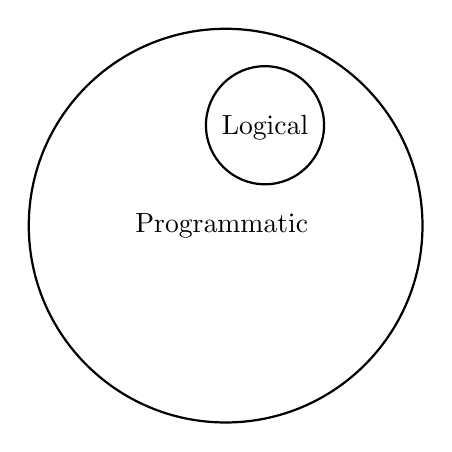
\begin{tikzpicture}[scale=2.5,cap=round,>=latex]    
    \draw[thick] (2.8cm,0cm) circle(1cm);
    \draw (2.78cm,0cm) node {Programmatic};
    \draw[thick] (3cm,0.51cm) circle(0.3cm);
    \draw (3cm,0.5cm) node {Logical};
  \end{tikzpicture}
\end{center}
To the following picture:
\begin{center}
  \begin{tikzpicture}[>=stealth',shorten >=1pt,auto,node distance=5 cm, scale = 1, transform shape]
    \node[state, minimum size=83.1pt] (A)              {Logical};
    \node[state] (B) [right of=A] {Programmatic};

    \path[->] (A) edge [bend left] (B)
              (B) edge [bend left] (A);
  \end{tikzpicture}    
\end{center}
We have seen this diagram before in the previous chapter, but there it
was used to give an intuitive understanding of the free speech
property, but the two fragments are not strictly separate.  Now we
insist that they are in fact strictly separate, and the first diagram
above is no longer applicable; unlike the freedom of speech language.
We will see that this separation allows for the lifting of most of the
value restrictions from the typing rules.

The freedom of speech language is not a very expressive programming
language.  For example, we did not show how to construct full
programs, nor did freedom of speech contain any notion of abstract
data types or pattern matching.  Thus, it is rather difficult to
consider freedom of speech as a real-world programming language.  In
this chapter we introduce the design of a new programming language
called Separation of Proof from Program ($\Sep$) that contains all of
these new features.  The logical and programmatic fragments are
strictly separate, and $\Sep$ is a full real-world programming
language complete with abstract datatypes and pattern matching.  There
are also additional features that we will introduce below.  The
definition of $\Sep$ is very large with over a hundred typing rules
and a large amount of syntax.  Therefore, we do not have the space to
introduce the complete definition in the same style as we did for
freedom of speech, but instead concentrate on the most important
aspects of the design.  If the reader wishes to wade through the
entire definition, then please see
Appendix~\ref{sec:annotated_separation_of_proof_from_program} and
Appendix~\ref{sec:unannotated_separation_of_proof_from_program}, but
the reader may wish to read this chapter first to understand the need
for two appendices.

$\Sep$ consists of two distinct phases: compile time and runtime, and
$\Sep$ separates each phase into its own language.  The compile time
phase uses the annotated $\Sep$ language, and the runtime phase uses
the unannotated $\Sep$ language\index{Separation of Proof from Program
  ($\Sep$)!Annotated Language}\index{Separation of Proof from Program
  ($\Sep$)!Unannotated Language}.  The former is then translated into
the second using an meta-level function called the eraser.  This
function removes the annotations from objects of the annotated
language yielding objects of the unannotated language, furthermore, the
eraser function removes all objects marked compile time, which
includes the entire proof language.  Thus to reiterate, the primary
goal of the annotated language is type checking and proving, while the
primary goal of the unannotated language is computation.  

The reader may suspect that the unannotated language most likely
consists primarily of the programmatic fragment, because if the proof
language is removed and has no computational content, then why keep it
around?  This is precisely correct, and an implementation of $\Sep$
would indeed do this, but we define an additional eraser function to
essentially translate the proof language of $\Sep$ into the
Curry-style version, that is a language with no annotations.  We
conjecture that the metatheory of $\Sep$ would be easier to carry out
in the unannotated language rather than the annotated one.  We do not
pursue this strand of thought further, but wanted to simply comment on
this notion. We do not define the eraser functions here, but the
interested reader can find their complete definitions at the end of
Appendix~\ref{sec:unannotated_separation_of_proof_from_program}.
Throughout the remainder of this chapter we will concentrate solely on
the annotated $\Sep$ language which we will just call $\Sep$.

\textbf{The overall picture.}  $\Sep$ consists of four main judgments:
\begin{center}
  \begin{tikzpicture}
    \matrix (m) [matrix of nodes,
                 row sep=3pt,
                 column 1/.style={anchor=base west},
                 column 2/.style={anchor=base},
                 column 3/.style={anchor=base east}
    ]
    {
      $[[D, G |- LK : Logical i]]$ & Super kinding.\\
      $[[D, G |- P : LK]]$         & Kinding.\\
      $[[D, G |- p : P]]$          & Proof typing.\\
      $[[D, G |- t : t']]$         & Program typing.\\ 
    };

    \draw [decoration={brace,amplitude=0.5em},decorate,ultra thick,gray]
        (m-1-1.north -| m.east) -- (m-3-1.south -| m.east);

        \draw [decoration={brace,amplitude=0.5em},decorate,ultra thick,gray]
        (m-4-1.north -| m.east) -- (m-4-1.south -| m.east);

    \node[draw=none] at (160pt,10.6pt) {Logical Fragment};
    \node[draw=none] at (177.8pt,-33.6pt) {Programmatic Fragment};
  \end{tikzpicture}  
\end{center}
As the previous table indicates the logical fragment is broken up into
three judgments.  This is because the language of the logical fragment
is no longer collapsed.  There are distinct languages for proofs,
predicates (types), kinds, and a new category we call super kinds.
Each of these will be discussed further below.  Now the programmatic
fragment consists of only a single judgment, because it has a
collapsed syntax very much like the freedom of speech language.  In
fact, the programmatic fragment is basically an extension of the
freedom of speech\index{Freedom of Speech} language, and so is not really that different. For
this reason we do not discuss the programmatic fragment in detail, but
only discuss a few important aspects of the fragment.  

In the freedom of speech language the connection between the two
fragments is very explicit.  The connection from the logical fragment
to the programmatic fragment is modeled by the $\Sepdrulename{Coerce}$
rule, and the connection from the programmatic fragment was modeled by
the dependent product types\index{Dependent Product Type}, which allowed arguments to functions to be
programs from the programmatic fragment.  However, $\Sep$ does not
have a coercion\index{Coercion} rule from the logical fragment to the programmatic
fragment.  Instead both fragments are related via the dependent
product types.  Logical programs are allowed to have programmatic
inputs, and programmatic programs are allowed to have logical
inputs.  

\textbf{The programmatic fragment.} The programmatic fragment can be
thought of as an extension of the programmatic fragment of the freedom
of speech language.  The extensions include datatypes, and pattern
matching.  There is one significant improvement to the programmatic
fragment over the freedom of speech language, and that is the lifting
of the value restrictions.  For example, the following are the
$\lambda$-abstraction and function application rules from the
programmatic fragment of $\Sep$:
\begin{center}
  \begin{mathpar}
    \SepdruleTRMXXLamPL{}  \and
    \SepdruleTRMXXLamMI{}  \and
    \SepdruleTRMXXApp{}    
  \end{mathpar}
\end{center}
We can see that these rules look very much like the rules of freedom
of speech, but there are some small differences.  First, we annotate
bound variables by their stage annotations.  This facilitates
reasoning as well as the definitions of the eraser
functions. Secondly, in the $\Sepdrulename{TRM\_LamPL}$ we annotate
the free variable $[[x]]$ in the context of the premise with the
$\mathsf{val}$ annotation.  This indicates that $[[x]]$ ranges over
programmatic values, and this is used to enforce
call-by-value\index{Call-by-value Reduction (CBV)}
applications. Compare this to the rule $\Sepdrulename{TRM\_LamMI}$
where $[[x]]$ does not only range over values, but also over diverging
terms.

These rules include the freedom of speech property\index{Freedom of Speech}.  The type $[[A]]$
is an alias for one of $[[t]]$, $[[P]]$, or $[[LK]]$, which means
compile-time functions -- using $\Sepdrulename{TRM\_LamMI}$ -- can
take in programmatic arguments, proof arguments, or even predicates.

Finally, the application rule $\Sepdrulename{TRM\_App}$ does not
contain any value restriction.  The argument $[[a]]$ ranges over
general terms, proofs, and predicates.  Thus, we have successfully
lifted the value restriction in the programmatic fragment.

\textbf{The logical fragment.}  We would now like to introduce the
logical fragment in some detail so the reader can get an idea of how
different it is from the logical fragment of the freedom of speech
language.  The syntax of the logical fragment of $\Sep$ is defined as
follows:

\begin{center}  
  \begin{math}
    \scriptsize
    \begin{array}{llllllllllllllll}      
      \begin{array}{lll}
      \text{(Super Kinds) } [[L]] ::= & [[Logical i]]\\
      & \\
      & \\
    \end{array}
    &
    \begin{array}{lllllll}           
      \text{(Logical Kind) } [[LK]] ::= 
      & [[x]] \\
      & \mid \mathsf{Formula}_{[[i]]} \\
      & \mid [[Forall x : A.LK]]\\
    \end{array}\\
    & \\
      \begin{array}{llllll}
        \text{(Predicates) } [[P]] ::= 
        & [[x]] \\
        & \mid [[\ L x : A . P]] \\
        & \mid [[P a]] \\
        & \mid [[Forall x : A . P]] \\
        & \mid [[let x = p in P]] \\
        & \mid [[let x = P in P']] \\
        & \mid [[let x = t [ p ] in P]] \\
        & \mid [[t1 = t2]] \\
        & \mid [[t !]] \\
        & \mid [[P1 + P2]] \\
        & \mid [[Exists x : A . P]] \\
        & \mid [[bot i]] \\
        & \mid [[t < t']] \\
        & \\
        & \\
        & \\
        & \\
        & \\
        & \\        
        & \\
        & \\
      \end{array}
      &
      \begin{array}{lll}
        \text{(Proofs) } [[p]] ::= 
        & [[x]] \\
        & \mid [[injl p with P]] \\
        & \mid [[injr p with P]] \\
        & \mid [[case p of x . p' , y . p'']] \\
        & \mid [[\ L x : A . p]] \\
        & \mid [[p a]] \\ 
        & \mid [[(a , p ) as P]] \\
        & \mid [[case p1 of ( x , y ) . p2]] \\
        & \mid [[let x = p' in p]] \\
        & \mid [[let x = P in p]] \\
        & \mid [[let x = t [ y ] in p]] \\
        & \mid [[join t1 t2]] \\
        & \mid [[conv p by q1 ... qn at x1 ... xm . P]] \\
        & \mid [[predconv p P]] \\
        & \mid [[valax t]] \\
        & \mid [[ord t t']] \\
        & \mid [[case t [ x ] p of R]] \\
        & \mid [[tcase t [ x ] of abort -> p1 | ! -> p2]] \\
        & \mid [[ind f x : t , p1 . p2]] \\
        & \mid [[contra p1]] \\
        & \mid [[contraval p1 p2]]\\
      \end{array}
    \end{array}
  \end{math}
\end{center}
Super kinds\index{Super Kind} are the types of logical kinds, which are themselves the
types of predicates.  Finally, predicates are the types of proofs.
The definition of the logical fragment is very reminiscent of the
definition of system $\Fw$\index{System $\Fw$} -- see
Section~\ref{sec:moderen_type_theory} for an introduction of $\Fw$.
In fact, predicates\index{Predicate} can be computed using $[[x]]$, $[[\ L x : A
. P]]$, $[[P a]]$, $[[let x = p in P]]$, $[[let x = P in P']]$, and
$[[let x = t [ p ] in P]]$; we have three different let expressions,
because of the strict separation of the various languages.  This
implies that the logical fragment is indeed a higher order language,
but a predicative one.  We have stratified the super kinds and logical
kinds into an infinite hierarchy of kinds.  We denote this by
$[[Logical i]]$ and $\mathsf{Formula}_{i}$.  This stratification is similar
to levels in SSF\index{Stratified System F (SSF)} -- see
Section~\ref{sec:moderen_type_theory} for more information on SSF.  

Now in comparison with the freedom of speech language we can see that
$\Sep$ has three new predicates: $[[t !]]$, $[[P1 + P2]]$, $[[Exists x
: A . P]]$, and $[[t < t']]$.  The first is called the termination
predicate and we will discuss this further below.  The second is the
type of sum types or, logically, the type for disjunction, and the third
is the type for existential quantification.  Note that we can
existentially quantify over logical kinds, predicates, proofs, and
terms.  Thus, the existential type\index{Existential Type} makes use of the freedom of speech
property similar to the dependent product type\index{Dependent Product
  Type}.  The final new
predicate is the structural ordering type $[[t < t']]$ which says that
$[[t]]$ is structurally smaller than $[[t']]$.  The structural
ordering type will be discussed further below.

The proof language is fairly straightforward, and is very similar to
the freedom of speech language with the addition of the necessary
proofs of the new predicates just discussed.  Thus, we do not go over
each proof construct.  The typing rules for logical kinds, predicates,
and proofs can be found in Figure~\ref{fig:logk-ty},
Figure~\ref{fig:pred-ty}, and Figure~\ref{fig:proofs-ty} respectively.
\begin{figure}
  \scriptsize
  \begin{mathpar}
    \SepdruleLKXXFormula{} \and
    \SepdruleLKXXPredicate{}
  \end{mathpar}
  \caption{Type-checking Rules for Logical Kinds}
  \label{fig:logk-ty}
\end{figure}
\begin{figure}
  \scriptsize
  \begin{mathpar}
    \SepdrulePRDXXVar{} \and
    \SepdrulePRDXXGD{} \and
    \SepdrulePRDXXBtm{} \and
    \SepdrulePRDXXDisj{} \and
    \SepdrulePRDXXForallOne{} \and
    \SepdrulePRDXXForallTwo{} \and
    \SepdrulePRDXXForallThree{} \and
    \SepdrulePRDXXForallFour{} \and
    \SepdrulePRDXXExtOne{} \and
    \SepdrulePRDXXExtTwo{} \and
    \SepdrulePRDXXExtThree{} \and
    \SepdrulePRDXXExtFour{} \and
    \SepdrulePRDXXLetPF{} \and
    \SepdrulePRDXXLetPRD{} \and
    \SepdrulePRDXXLet{} \and
    \SepdrulePRDXXKXXEq{} \and
    \SepdrulePRDXXTRM{} \and
    \SepdrulePRDXXLam{} \and
    \SepdrulePRDXXApp{}
  \end{mathpar}
  \caption{Type-checking Rules for Predicates}
  \label{fig:pred-ty}
\end{figure}
\begin{figure}
  \scriptsize
  \begin{mathpar}
    \SepdrulePRFXXVar{} \and
    \SepdrulePRFXXGD{}  \and
    \SepdrulePRFXXExti{}  \and
    \SepdrulePRFXXExtE{}  \and
    \SepdrulePRFXXInl{} \and
    \SepdrulePRFXXInr{} \and
    \SepdrulePRFXXOrElim{} \and
    \SepdrulePRFXXFT{} \and
    \SepdrulePRFXXFPRD{} \and
    \SepdrulePRFXXFLK{} \and
    \SepdrulePRFXXApp{} \and
    \SepdrulePRFXXLetPRF{} \and
    \SepdrulePRFXXLetPRD{} \and
    \SepdrulePRFXXLet{} \and
    \SepdrulePRFXXJoin{} \and
    \SepdrulePRFXXConv{} \and
    \SepdrulePRFXXPRDConv{} \and
    \SepdrulePRFXXVal{} \and
    \SepdrulePRFXXOrd{} \and
    \SepdrulePRFXXInd{} \and
    \SepdrulePRFXXCTROne{} \and
    \SepdrulePRFXXCTRTwo{} \and
    \SepdrulePRFXXCTRV{} \and
    \SepdrulePRFXXCase{} \and
    \SepdrulePRFXXTCase{} 
  \end{mathpar}
  \caption{Type-checking Rules for Proofs}
  \label{fig:proofs-ty}
\end{figure}
The reader may wish to look over the typing rules for proofs to get an
idea of which proof construct introduces each of the new predicates.

\textbf{The termination prediate.}  In the freedom of speech language
if one wanted to prove that a programmatic program is terminating one
simply had to define it in the logical fragment, but this is not
possible in $\Sep$, because of the strict separation of the logical
and programmatic fragments.  The termination predicate adds the
ability to prove programmatic programs terminating.  The termination
predicate is denoted $[[t !]]$, and can be read as the program $[[t]]$
terminates at a value.  We prove $[[t !]]$ using the rule
$\Sepdrulename{PRF\_Val}$:
\[ \SepdrulePRFXXVal{} \] This rule says, that if we can show $[[D, G
|- val t]]$, then we can prove $[[t !]]$.  We call the judgment $[[D,
G |- val t]]$ the semantic value judgment.  If it holds, then $[[t]]$
is either an actual syntactic value, a free variable annotated in the
context as ranging over values, or a termination cast.  See
Figure~\ref{fig:sem-val} for the definition of the semantic value
judgment.
\begin{figure}
  \begin{mathpar}
    \SepdruleVXXVar{} \and
    \SepdruleVXXType{} \and
    \SepdruleVXXPi{} \and
    \SepdruleVXXLamPlus{} \and
    \SepdruleVXXLamMinus{} \and
    \SepdruleVXXRec{} \and
    \SepdruleVXXCtor{} \and
    \SepdruleVXXtCast{}
  \end{mathpar}
  \caption{Semantic Values}
  \label{fig:sem-val}
\end{figure}
One may feel that the rule $\Sepdrulename{PRF\_Val}$ is a bit
restrictive.  This rule is supposed to allow the proof that a
terminating program is indeed terminating, but on the nose it seems
that the only things we can prove are terminating are semantic
values, which are trivially terminating.  However, this is not the
case.  If one can prove that $[[t]]$ is terminating for some non-value
$[[t]]$, then one must have constructed the value of $[[t]]$, say
$[[v]]$.  Now it is trivially the case that $[[t]]$ and $[[v]]$ are
joinable, thus using $\Sepdrulename{PRF\_Join}$ we can prove $[[t =
v]]$.  In addition, since we know $[[v]]$ is a value, then we can
prove that it is a semantic value trivially.  Thus, using these two
proofs we can then prove $[[D, G |- valax v : t !]]$ using the rules
$\Sepdrulename{PRF\_Val}$ and $\Sepdrulename{PRF\_Conv}$.

The termination cast is a means of casting programs to values if they
can be proven to be terminating.  That is, any terminating program may
be treated as a value. Lets consider the introduction rule for
the termination cast:
\[ 
\SepdruleTRMXXtCast{}
\]
This rules states that if we have a well-typed $[[t]]$ of type
$[[t']]$, and a proof $[[p]]$ that $[[t]]$ terminates, that is of type
$[[t !]]$, then we may cast $[[t]]$ to a value denoted $[[tcast t by
p]]$ which is also of type $[[t']]$.  

There is one final component of the termination predicate called the
termination case expression.  This is an expression that amounts to
computationally case splitting over the termination behavior of a
program.  Now do not be alarmed!  This does not imply that this is a
proof of the halting problem.  Consider the typing rule for the
termination case expression: \[ \SepdrulePRFXXTCase{} \] This rule
status that if $[[t]]$ terminates then execute the second branch
$[[p2]]$, which is allowed to use the proof showing that $[[t]]$
terminates, otherwise if $[[t]]$ is diverges -- here we model
divergence using $[[abort t']]$ -- then execute the first branch
$[[p1]]$ which is allowed to use the proof showing $[[t]]$ is
equivalent to $[[abort t']]$.  Now computationally speaking this rule
is undecidable.  It is impossible to take an arbitrary program and
decide whether it diverges or not, but adding this axiom is not
inconsistent, because it simply captures the notion that either a
program terminates or it diverges, and this is no more inconsistent
then adding the law-of-excluded middle to our logic.  In fact, one
might expect that adding termination case could imply the
law of excluded middle\index{Law of Excluded Middle (LEM)}
making our logic classical, but this is an open problem.

\textbf{Structural ordering.}  There is one final interesting feature
that sets $\Sep$ apart from the freedom of speech language, and many
others.  Recall that in the freedom of speech language the logical
fragment contained a terminating recursor, but the recursive argument
had to be a natural number.  $\Sep$ relaxes this requirement to an
arbitrary datatype by introducing a new predicate called the
structural order denoted $[[t < t']]$.  Intuitively, if $[[t]]$ is a
well-defined strict subexpression of $[[t']]$, then we may conclude
$[[t < t']]$.  The rule for introducing the structural order predicate
is as follows: \[ \SepdrulePRFXXOrd{} \] This rule is very much like
the rule for introducing the termination predicate in that it is
defined for values only, however, when mixed with equality it can be
very powerful.  The judgment $[[t subexpp t']]$ is the subexpression
ordering on datatype constructors.  See
Appendix~\ref{sec:annotated_separation_of_proof_from_program} for the
complete definition.  

The structural order predicate is then used in the definition of
induction in the logical fragment: \[ \SepdrulePRFXXInd{} \] As we can
see the inductive call must be given a proof that the argument we are
inducting over has structurally decreased.  This means that we can now
do induction on many different types of data, for example, lists,
trees, natural numbers, and any other inductively defined data.

Throughout this chapter we have seen only the positive perspective of
the design of $\Sep$.  So now we briefly discuss one major lesson
learned from this design.  Relaxing the value restrictions was
achieved by a strict separation of the logical and programmatic
fragments.  In addition, the proof language has been separated into
several different languages.  This strict separation prevents code
reuse.  That is, there are functions that can be written in both the
programmatic fragment and the logical fragment, but these have to be
written twice.  Thus, through the strict separation we have gained no
value restrictions, but lost code reuse.  This is the major drawback
of the $\Sep$ design.  

In this chapter we introduced a new dependently-typed functional
programming language called Separation of Proof from Program.  $\Sep$
is a large advancement over the freedom of speech language.  It has
several new predicates for disjunction, existential quantification,
termination, and structural ordering.  In addition $\Sep$ contains the
freedom of speech property, but is designed so as to prevent the need
for the value restrictions we have in the freedom of speech language.
Thus, programming in $\Sep$ is more enjoyable.  Lastly, $\Sep$
contains inductive datatypes with pattern matching.  Therefore,
real-world programming examples can be carried out in $\Sep$; in fact,
several examples can be found in the paper \cite{Kimmel:2012}.
